\documentclass[aspectratio=169]{beamer}

% Theme and color settings
\usetheme{Madrid}
\usecolortheme{whale}
\usefonttheme{structurebold}

% Additional packages
\usepackage{booktabs}
\usepackage{amsmath}
\usepackage{graphicx}
\usepackage{tabularx}
\usepackage{multirow}
\usepackage{tikz}
\usetikzlibrary{shapes.geometric, arrows, positioning}

% Title page information
\title{Análisis del Rendimiento de Funciones C en Diferentes Arquitecturas y Compiladores}
\subtitle{CI0131 - Diseño de Experimentos}
\date{\today}
\institute{Universidad de Costa Rica}

\begin{document}

% Title page
\begin{frame}
    \titlepage
\end{frame}

% Table of contents
\begin{frame}{Contenido}
    \tableofcontents
\end{frame}

\section{Descripción del Problema}

\begin{frame}{Problema de Investigación}
    \begin{block}{Contexto}
        En el dominio del desarrollo de software de alto rendimiento, la elección de la arquitectura y el compilador ejerce una influencia sustancial en el tiempo de ejecución y el uso de recursos.
    \end{block}
    
    \begin{block}{Propósito}
        Cuantificar el impacto de estas variables y su relación a través de metodologías de diseño y análisis de experimentos, proporcionando información valiosa para la toma de decisiones en proyectos de ingeniería de software.
    \end{block}
\end{frame}

\section{Hipótesis y Objetivos}

\begin{frame}{Hipótesis y Objetivos}
    \begin{block}{Pregunta de Investigación}
        ¿Cuál es el efecto principal de la arquitectura de la CPU y el compilador en el rendimiento de funciones en C?
    \end{block}
    
    \begin{block}{Objetivos}
        \begin{itemize}
            \item Medir el desempeño de ejecución de las funciones seleccionadas en diferentes combinaciones de arquitectura y compilador.
            \item Analizar la influencia de la arquitectura y el compilador en la variabilidad del desempeño de funciones.
        \end{itemize}
    \end{block}
\end{frame}

\section{Variable de Respuesta}

\begin{frame}{Variable de Respuesta: Descriptivo}
    \begin{table}
        \begin{tabularx}{\textwidth}{|>{\raggedright\arraybackslash}p{2cm}|>{\raggedright\arraybackslash}X|>{\raggedright\arraybackslash}X|>{\raggedright\arraybackslash}p{2cm}|>{\raggedright\arraybackslash}p{2cm}|}
            \hline
            \textbf{Nombre} & \textbf{Descripción} & \textbf{Justificación} & \textbf{Tipo} & \textbf{Unidades} \\
            \hline
            T\_exec & Tiempo transcurrido desde el inicio hasta el fin de la ejecución del binario compilado de la función & En esta variable almacenamos del tiempo de ejecución de la batería de pruebas & Continua & Milisegundos \\
            \hline
        \end{tabularx}
    \end{table}
\end{frame}

\begin{frame}{Variable de Respuesta: Metodológico}
    \begin{table}
        \begin{tabularx}{\textwidth}{|>{\raggedright\arraybackslash}p{2cm}|>{\raggedright\arraybackslash}X|>{\raggedright\arraybackslash}p{2cm}|>{\raggedright\arraybackslash}X|}
            \hline
            \textbf{Nombre} & \textbf{Metodología de recolección} & \textbf{Rango} & \textbf{Precisión y Exactitud} \\
            \hline
            T\_exec & Se ejecutará cada función con medición de tiempo utilizando herramientas como time, perf o el mismo clock del sistema operativo, Tras investigación exploratoria se decidirá si cada medición será repetida 5 veces para disminuir posibles sesgos, o solo 1 vez si vemos que no es factible repetirlo 5 veces. & 0 ms – 100,000 ms & \textbf{Exactitud:} Repetir 100 ejecuciones de manera secuencial para cuantificar variabilidad. \newline \textbf{Precisión:} calcular la desviación estándar de las ejecuciones anteriormente mencionadas. \\
            \hline
        \end{tabularx}
    \end{table}
\end{frame}

\section{Unidad Experimental}

\begin{frame}{Unidad Experimental}
    \begin{table}
        \begin{tabularx}{\textwidth}{|>{\raggedright\arraybackslash}p{2cm}|>{\raggedright\arraybackslash}X|>{\raggedright\arraybackslash}X|>{\raggedright\arraybackslash}p{2cm}|>{\raggedright\arraybackslash}p{1.5cm}|}
            \hline
            \textbf{Nombre} & \textbf{Descripción} & \textbf{Justificación} & \textbf{Tipo} & \textbf{Unidades} \\
            \hline
            Función C & Función escrita en lenguaje C que implementa una lógica específica y que será compilada y ejecutada. & La función en C es la unidad fundamental sobre la cual se medirá el rendimiento, ya que permite evaluar directamente el impacto de la arquitectura y el compilador sobre un código idéntico. & Discreta categórica & N/A \\
            \hline
        \end{tabularx}
    \end{table}
\end{frame}

\section{Factores de Diseño}

\begin{frame}{Factores de Diseño: Descriptivo}
    \begin{table}
        \begin{tabularx}{\textwidth}{|>{\raggedright\arraybackslash}p{2.5cm}|>{\raggedright\arraybackslash}X|>{\raggedright\arraybackslash}X|>{\raggedright\arraybackslash}X|>{\raggedright\arraybackslash}p{2.5cm}|}
            \hline
            \textbf{Nombre} & \textbf{Descripción} & \textbf{Justificación de inclusión} & \textbf{Justificación como factor de diseño} & \textbf{Tipo y unidades} \\
            \hline
            Arquitectura CPU & Plataforma hardware utilizada para ejecutar el binario & Afecta el rendimiento por diferencias de arquitecture (ej:manejo de memoria)& Fundamental para probar la hipótesis de variabilidad entre plataformas & Discreta categórica (intel, amd) \\
            \hline
            Compilador & Herramienta utilizada para generar el binario de la función & Diferentes optimizaciones afectan el desempeño & Necesario para medir la influencia del compilador en el rendimiento & Discreta categórica (GCC, Clang) \\
            \hline
        \end{tabularx}
    \end{table}
\end{frame}

% Página 1: Arquitectura CPU
\begin{frame}{Factores de Diseño: Metodológico - Arquitectura CPU}
    \small
    \begin{table}
        \begin{tabularx}{\textwidth}{|>{\raggedright\arraybackslash}p{2cm}|>{\raggedright\arraybackslash}X|>{\raggedright\arraybackslash}p{1.5cm}|>{\raggedright\arraybackslash}p{1cm}|>{\raggedright\arraybackslash}p{2.5cm}|>{\raggedright\arraybackslash}X|}
            \hline
            \textbf{Nombre} & \textbf{Metodología} & \textbf{Rango} & \textbf{Niveles} & \textbf{Justificación} & \textbf{Precisión y exactitud} \\
            \hline
            Arquitectura CPU & Uso de hardware real para cada arquitectura para eliminar el overhead de un emulador & intel i7, amd & 2 & Representan arquitecturas populares, relevantes y contemporáneas entre ellas & \textbf{Precisión:} cambiar físicamente de máquina limpia en < 1 min. \textbf{Exactitud:} comprobar frecuencia nominal con lscpu y tolerancia ±1\%. \\
            \hline
        \end{tabularx}
    \end{table}
\end{frame}

% Página 2: Compilador
\begin{frame}{Factores de Diseño: Metodológico - Compilador}
    \small
    \begin{table}
        \begin{tabularx}{\textwidth}{|>{\raggedright\arraybackslash}p{2cm}|>{\raggedright\arraybackslash}X|>{\raggedright\arraybackslash}p{1.5cm}|>{\raggedright\arraybackslash}p{1cm}|>{\raggedright\arraybackslash}p{2.5cm}|>{\raggedright\arraybackslash}X|}
            \hline
            \textbf{Nombre} & \textbf{Metodología} & \textbf{Rango} & \textbf{Niveles} & \textbf{Justificación} & \textbf{Precisión y exactitud} \\
            \hline
            Compilador & Selección del compilador instalado apropiadamente para cada arquitectura & GCC, Clang & 2 & Ambos son cornerstones de los compiladores C opensource & \textbf{Exactitud:} validar con gcc --version y clang --version. \textbf{Precisión:} repetir compilación 5 veces (verificar durante EDA si es factible o no), verificar hash idéntico y tamaño ±0 bytes. \\
            \hline
        \end{tabularx}
    \end{table}
\end{frame}

\section{Factores Constantes}

\begin{frame}{Factores que se Mantendrán Constantes: Descriptivo}
    \begin{table}
        \begin{tabularx}{\textwidth}{|>{\raggedright\arraybackslash}p{2cm}|>{\raggedright\arraybackslash}X|>{\raggedright\arraybackslash}X|>{\raggedright\arraybackslash}X|>{\raggedright\arraybackslash}p{2cm}|}
            \hline
            \textbf{Nombre} & \textbf{Descripción} & \textbf{Justificación de inclusión} & \textbf{Justificación como factor constante} & \textbf{Tipo y unidades} \\
            \hline
            Código fuente & Funciones escritas en C & Garantizar comparabilidad & Para atribuir diferencias únicamente a arquitectura o compilador & N/A \\
            \hline
        \end{tabularx}
    \end{table}
\end{frame}

\begin{frame}{Factores que se Mantendrán Constantes: Metodológico}
    \small
    \begin{table}
        \begin{tabularx}{\textwidth}{|>{\raggedright\arraybackslash}p{2cm}|>{\raggedright\arraybackslash}X|>{\raggedright\arraybackslash}p{1.5cm}|>{\raggedright\arraybackslash}p{1cm}|>{\raggedright\arraybackslash}X|>{\raggedright\arraybackslash}X|}
            \hline
            \textbf{Nombre} & \textbf{Metodología de fijación} & \textbf{Rango} & \textbf{Nivel} & \textbf{Justificación} & \textbf{Precisión y exactitud} \\
            \hline
            Sistema operativo & Se usará la misma versión del sistema operativo entre ejecuciones de pruebas & ubuntu 24.02 & 1 & No es parte del experimento probar diferentes sistemas operativos & Chequeo previo con lsb\_release cada día de prueba. \\
            \hline
            Versión del compilador e flags & Usar misma versión del compilador y mismo comando & gcc 15.1 & 1 & Para aislar efecto del compilador puro sin variación de flags & Script automatizado que imprime versión y flags antes de cada corrida. \\
            \hline
            Cantidad de programas en primer plano & Solo estara ejecutandose las pruebas en primer plano & 1 & 1 & Lo ideal es tener la misma carga de trabajo en todas las pruebas & Medir uso de CPU y RAM antes de cada bloque; debe ser ≤ 5\% \\
            \hline
        \end{tabularx}
    \end{table}
\end{frame}

\section{Factores Variables}

\begin{frame}{Factores a los que se Permitirá Variar}
    \begin{table}
        \begin{tabularx}{\textwidth}{|>{\raggedright\arraybackslash}p{2cm}|>{\raggedright\arraybackslash}X|>{\raggedright\arraybackslash}X|>{\raggedright\arraybackslash}X|>{\raggedright\arraybackslash}p{2.5cm}|}
            \hline
            \textbf{Nombre} & \textbf{Descripción} & \textbf{Justificación de inclusión} & \textbf{Justificación como factor variable} & \textbf{Tipo y unidades} \\
            \hline
            Carga del sistema & Procesos en segundo plano y uso de recursos del sistema & La carga del sistema puede afectar los tiempos de ejecución & No se controlará para reflejar condiciones más realistas de uso en producción & Continua (\% de uso de CPU/memoria) \\
            \hline
            Temperatura de CPU & Temperatura del procesador & La temperatura puede influir en el rendimiento& Representar condiciones reales de operación & Continua (°C) \\
            \hline
            Tamaño de datos & Volumen de datos procesados por la función & Puede afectar los patrones de acceso a memoria y caché & Se medirá su efecto pero no se controlará estrictamente & Discreta numérica (bytes) \\
            \hline
        \end{tabularx}
    \end{table}
\end{frame}

\section{Factores de Molestia}

\begin{frame}{Factores de Molestia}
    \small
    \begin{table}
        \begin{tabularx}{\textwidth}{|>{\raggedright\arraybackslash}p{2.5cm}|>{\raggedright\arraybackslash}X|>{\raggedright\arraybackslash}X|>{\raggedright\arraybackslash}X|>{\raggedright\arraybackslash}p{2cm}|}
            \hline
            \textbf{Nombre} & \textbf{Descripción} & \textbf{Justificación de inclusión} & \textbf{Estrategia de minimización} & \textbf{Tipo y unidades} \\
            \hline
            Código con librerías dinámicas & Bibliotecas compartidas cargadas en tiempo de ejecución & Pueden variar la latencia de enlace dinámico & USar herramientas como prelink& Categórica (sí/no) \\
            \hline
            Interrupciones de CPU y cambios de contexto & Eventos de sistema que detienen el proceso y redistribuyen tiempo CPU & Alteran mediciones de tiempo de ejecución & Se registran con perf record y se aleatoriza el orden de pruebas & Continua (eventos/minuto) \\
            \hline
            Materiales y enfriamiento (throttling térmico) & Temperatura del procesador durante la ejecución & La temperatura puede influir en el rendimiento & Se permite variar naturalmente para representar condiciones reales & Continua (°C) \\
            \hline
        \end{tabularx}
    \end{table}
\end{frame}

\section{Restricciones y Diseño}

\begin{frame}{Restricciones}
    \begin{itemize}
        \item Solo se disponen de dos máquinas físicas (Intel y AMD)
        \item No se probarán sistemas operativos ni flags adicionales
        \item Máximo de 5 ejecuciones por combinación debido a tiempo computacional (se tiene que averiguar durante EDA si es factible a nivel de tiempo)
        \item No se incluyen arquitecturas virtuales/emuladas
    \end{itemize}
\end{frame}

\begin{frame}{Aspectos de Diseño}
    \begin{itemize}
        \item Diseño factorial $2^2$ (2 arquitecturas × 2 compiladores)
        \item Dos réplicas completas (10 ejecuciones por combinación)
        \item Aleatorización: orden aleatorio de las corridas
    \end{itemize}
    
    \begin{figure}
        \centering
        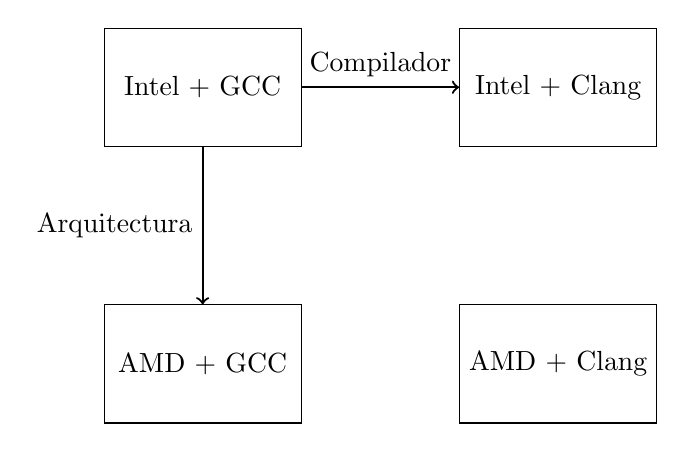
\begin{tikzpicture}[node distance=2cm]
            \node (intel_gcc) [draw, rectangle, minimum width=2.5cm, minimum height=1.5cm] {Intel + GCC};
            \node (intel_clang) [draw, rectangle, minimum width=2.5cm, minimum height=1.5cm, right=of intel_gcc] {Intel + Clang};
            \node (amd_gcc) [draw, rectangle, minimum width=2.5cm, minimum height=1.5cm, below=of intel_gcc] {AMD + GCC};
            \node (amd_clang) [draw, rectangle, minimum width=2.5cm, minimum height=1.5cm, right=of amd_gcc] {AMD + Clang};
            
            \draw[->,thick] (intel_gcc) -- (intel_clang) node[midway,above] {Compilador};
            \draw[->,thick] (intel_gcc) -- (amd_gcc) node[midway,left] {Arquitectura};
        \end{tikzpicture}
        \caption{Diseño factorial $2^2$}
    \end{figure}
\end{frame}

\begin{frame}{Corridas de Prueba}
    \begin{itemize}
        \item Se realizara pruebas preliminares con 10 funciones de prueba para verificar scripts de automatización y medición (ademas de la EDA)
        \item Ajustes realizados:
        \begin{itemize}
            \item Confirmación de sincronización de relojes
            \item Limpieza de caché entre ejecuciones
        \end{itemize}
        \item No hay datos de interés adicional para el experimento principal
    \end{itemize}
\end{frame}


\section{Conclusión}

\begin{frame}{Conclusión y Siguientes Pasos}
    \begin{block}{Valor esperado del estudio}
        Este experimento proporcionará información cuantitativa sobre:
        \begin{itemize}
            \item Efectos principales de arquitectura y compilador en el rendimiento
            \item Posibles interacciones entre estos factores
            \item Variabilidad del rendimiento bajo condiciones controladas
        \end{itemize}
    \end{block}
    
    \begin{block}{Aplicaciones prácticas}
        Los resultados pueden informar decisiones de:
        \begin{itemize}
            \item Selección de hardware para desarrollo de software
            \item Elección de compilador según el caso de uso
            \item Estimación de rendimiento en diferentes entornos
        \end{itemize}
    \end{block}
\end{frame}

\begin{frame}[standout]
    ¡Gracias por su atención!
    
    ¿Preguntas?
\end{frame}

\end{document}